\chapter{Methods and Experiments} \label{methods-and-experiments}

\section{Single-Agent Bilateral Negotiation Environment (\gls{sbe})}
In this environment, agent represents the negotiator in negotiation mechanism.

\subsection{Independent Negotiator in NegMAS}
In the environment has just single learnable \gls{drl} negotiator. All \gls{rl} algorithms with discrete action space can be tested in this specific environment. In the experiment of this thesis, \gls{dqn} and \gls{ppo} were tested in four learning cases:
\begin{itemize}
	\item single issue, acceptance strategy
	\item single issue, offer strategy
	\item multi-issues, acceptance strategy
	\item multi-issues, offer startegy
\end{itemize}

The training step of DQN is shown in Figure \ref{fig:dqn}
\begin{figure}[htbp]
\centering
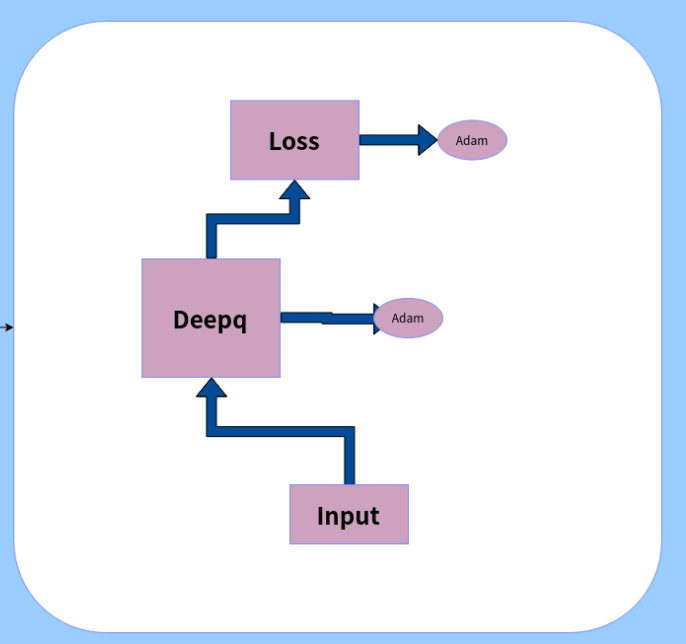
\includegraphics[width=0.40\textwidth]{./images/dqn.png}
\caption{Training step of DQN}
\label{fig:dqn}
\end{figure}

\subsection{Experiment} \label{sbe:experiment}
Figure \ref{fig:bilateral-negotiation} diagrams the Game in \gls{sbe}
\begin{figure}[htbp]
\centering
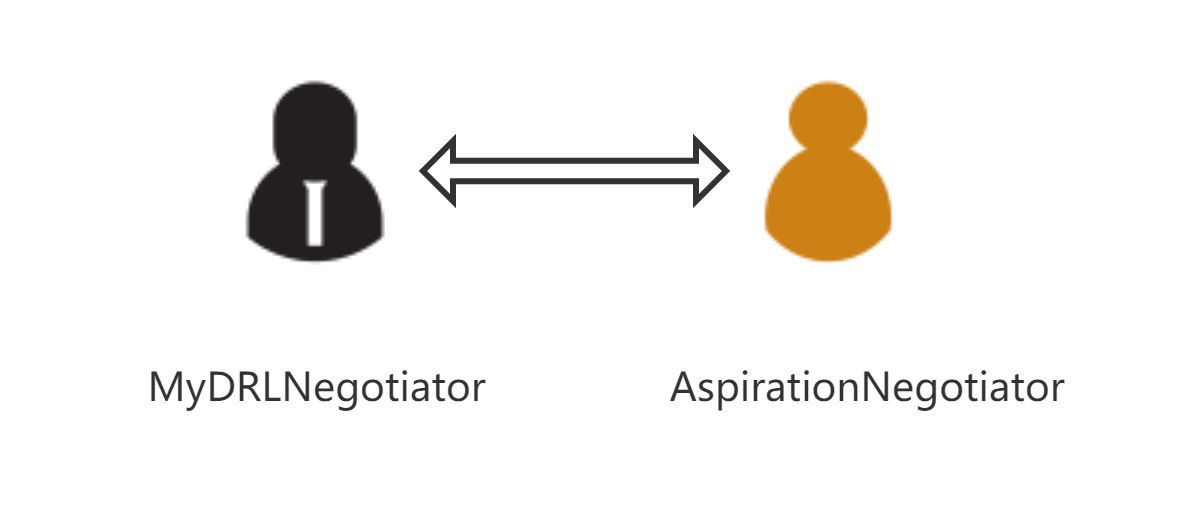
\includegraphics[width=0.50\textwidth]{./images/bilateral-negotiation.png}
\caption{Bilateral Negotiation Game in \gls{sbe}, My Deep Reinforcement Learning Negotiator vs. Aspiration Negotiator}
\label{fig:bilateral-negotiation}
\end{figure}

\subsubsection{single issue}
Negotiation mechanism is \gls{saom}, split the learning strategy as two parts, acceptance strategy and offer strategy, 

Acceptance strategy: actions of agent are \texttt{Accept offer}, \texttt{Wait} and \texttt{Reject offer}. Observation of agent are offer of opponent and current time(running time, or current step of negotiation). Algorithms are \gls{dqn} (blue) and \gls{ppo} (red). Mean episode reward is shown in \ref{fig:acceptance-single-issue}

Offer strategy: Actions of negotiator are all outcomes set in mechanism. The observation is same as defined in the acceptance strategy. Before training the agent, normalize action and observation. Algorithm is DQN and PPO.

\begin{figure}[htbp]
\centering
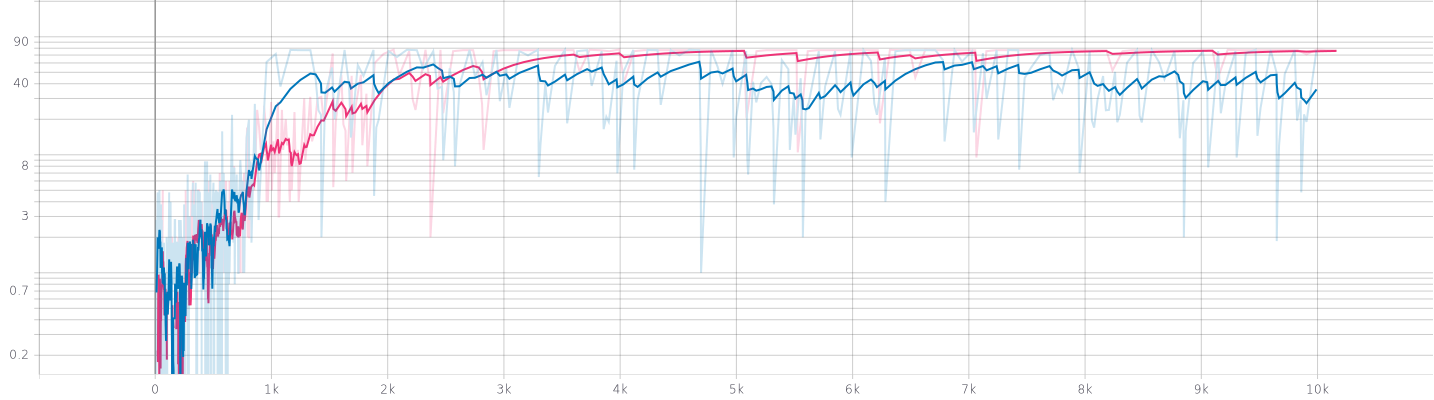
\includegraphics[width=0.80\textwidth]{./images/ac_s_dqn_ppo1_log_EpRe.png}
\caption{Episode mean reward of acceptance strategy under single issue}
\label{fig:acceptance-single-issue}
\end{figure}

\subsubsection{multi issues}

\subsection{Evaluation}

\section{Multi-Agent Concurrent Bilateral Negotiation Environment (\gls{mcbe})}
In this environment, agent represents the factory manager and negotiation controller in standard \gls{scml} and \gls{scml} OneShot, respectively.

The agent interacting with environment may be have many related trainable agents as the part of learner(e.g. one seller, one buyer) in the model. The detail of interactive logic is shown below in \ref{fig:interacting-logic-maddpg-scml}

\begin{figure}[htbp]
\centering
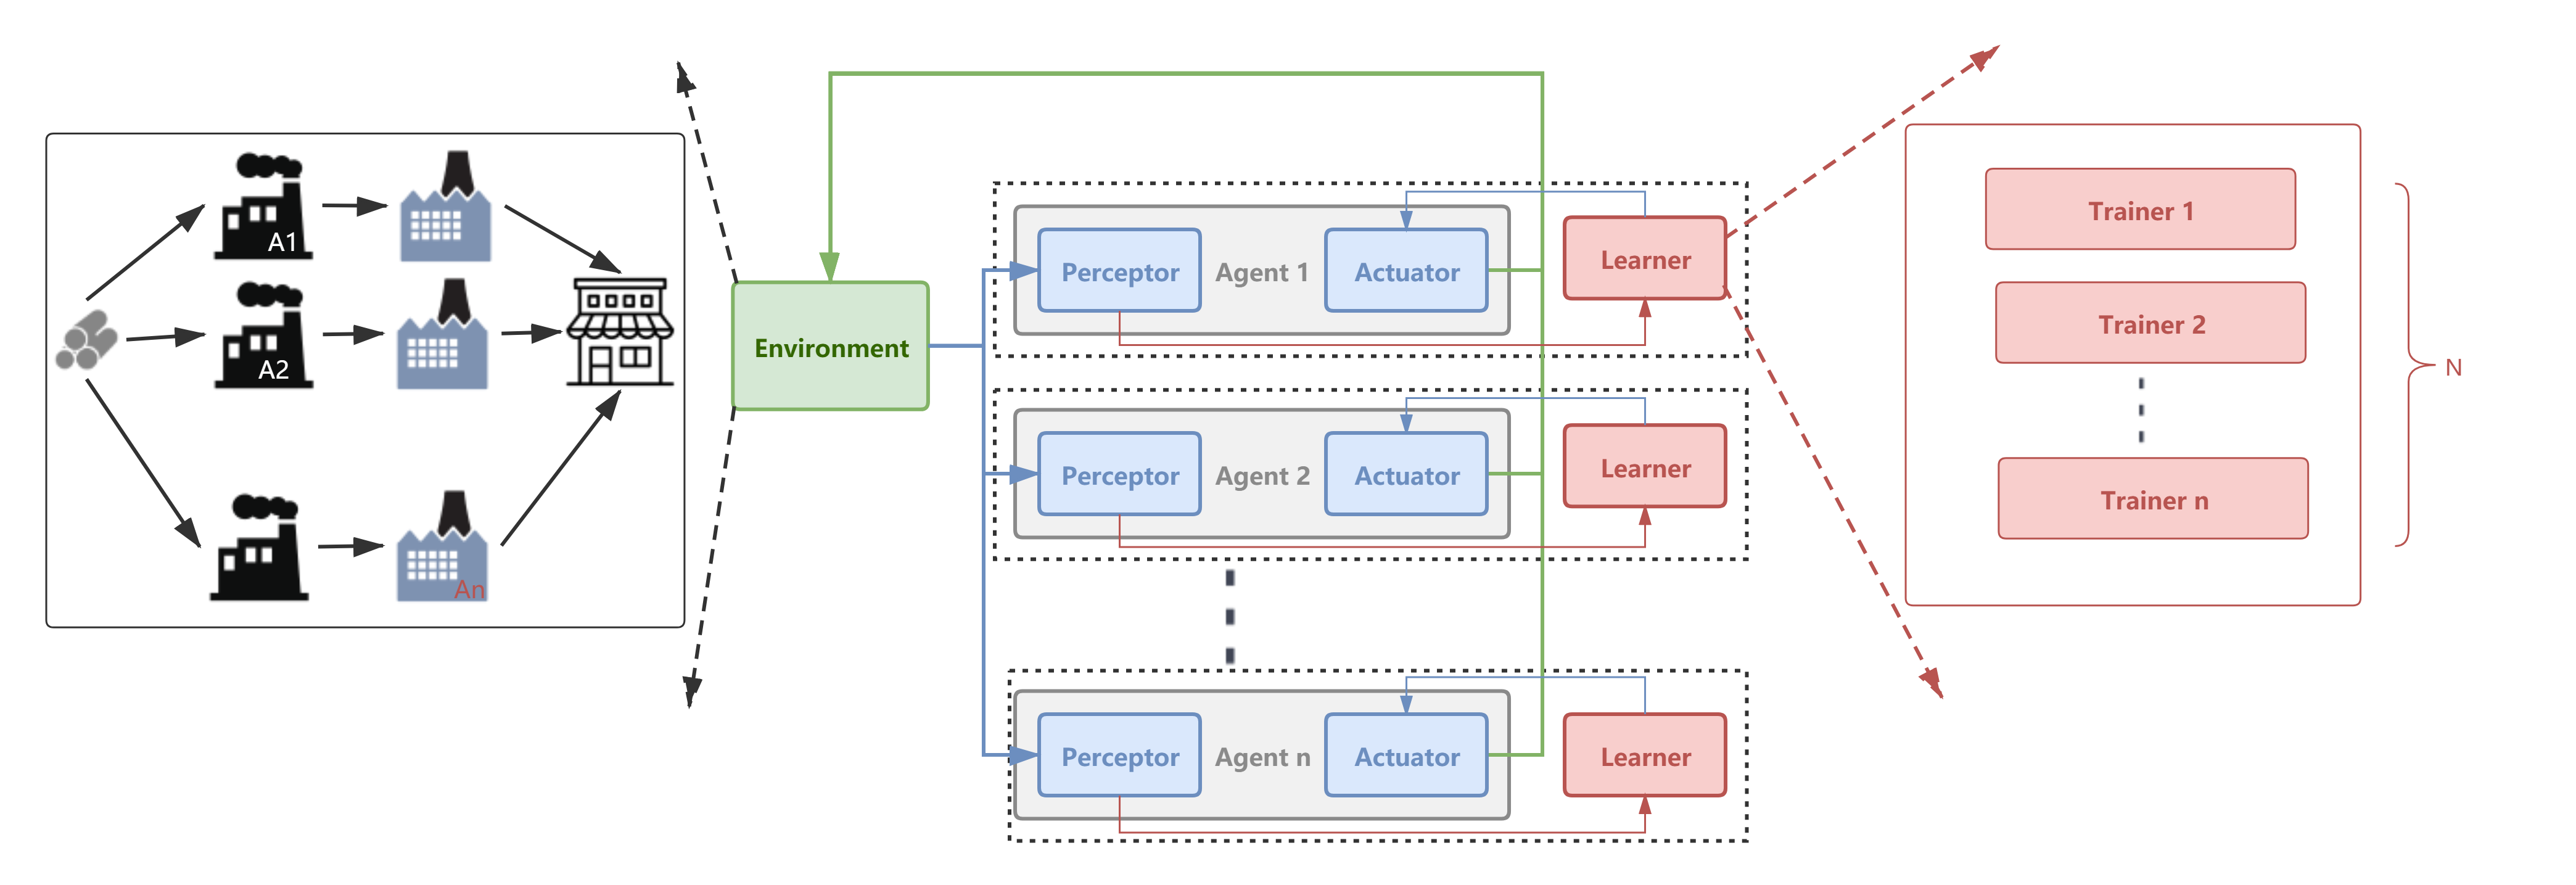
\includegraphics[width=1.0\textwidth]{./images/scnk.png}
\caption{Interactive logic based on the perspective of \gls{scml}. N: The maximum number of concurrent negotiations for a single agent}
\label{fig:interacting-logic-maddpg-scml}
\end{figure}
\subsection{\gls{maddpg} in \gls{scml}} \label{methods:maddpg}
Shown in \ref{fig:method-maddpg-scml}

\begin{figure}[htbp]
\centering
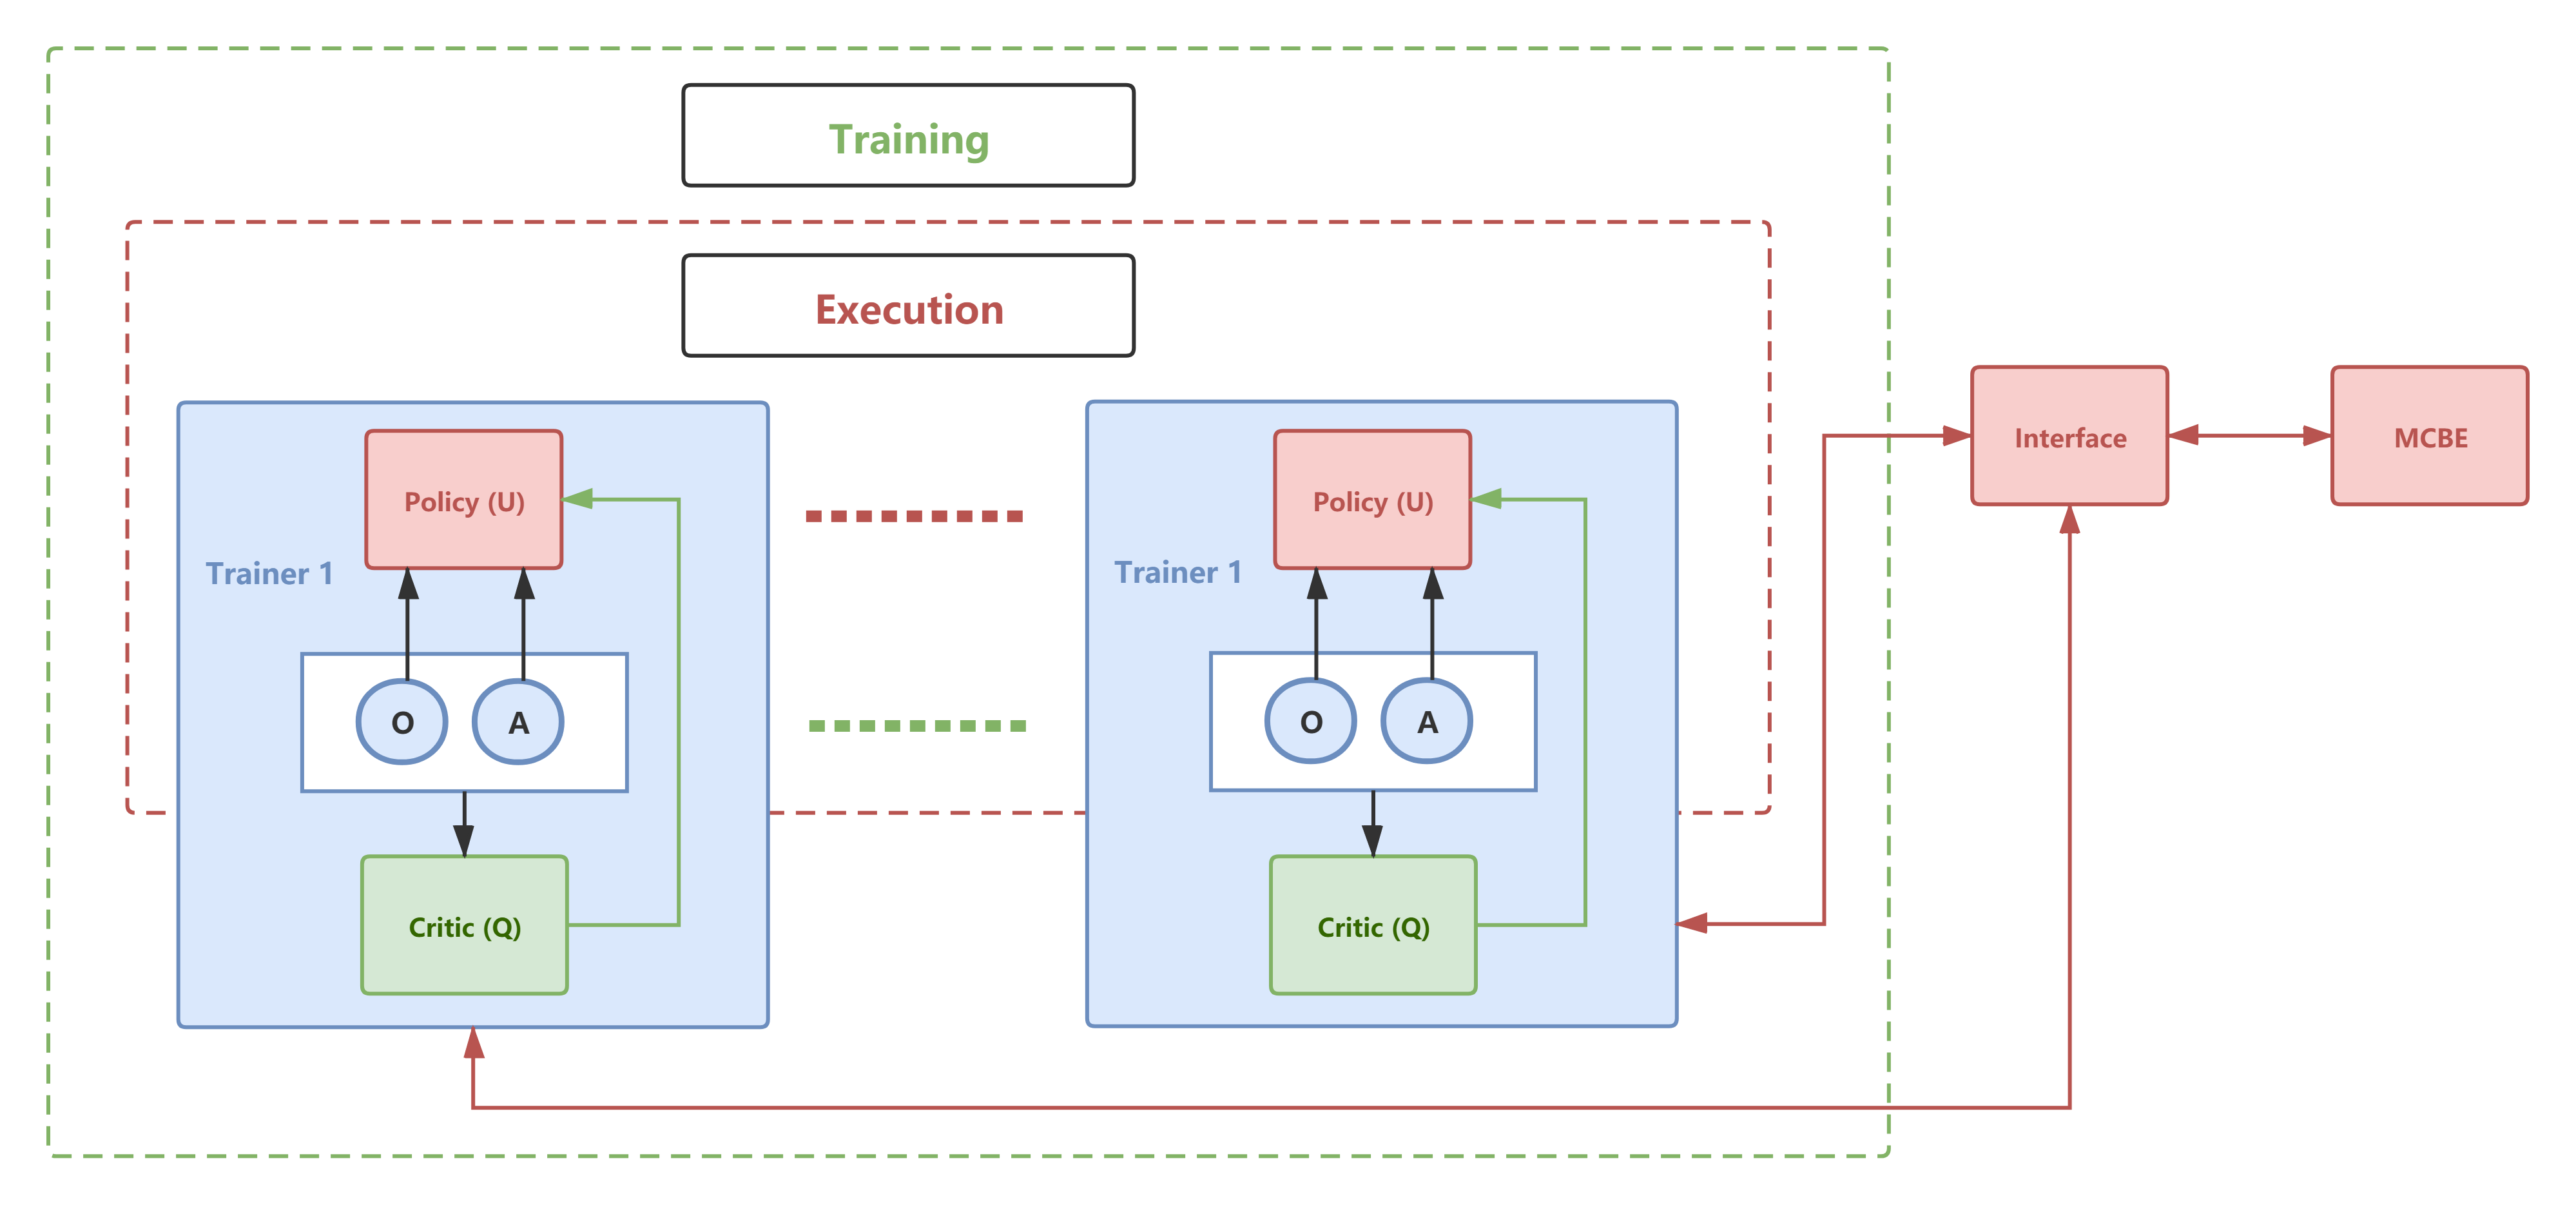
\includegraphics[width=0.80\textwidth]{./images/scml-maddpg.png}
\caption{\gls{maddpg} used in \gls{mcbe}}
\label{fig:method-maddpg-scml}
\end{figure}
Actors output actions as inputs to related agents interacting with the environment. Agents interacting with environment outputs the observation and reward as the inputs to related agents trained in the model. 

\begin{algorithm}[H]
  \SetAlgoLined
  \KwData{this text}
  \KwResult{how to write algorithm with \LaTeX2e }

  initialization\;
  \While{not at end of this document}{
    read current\;
    \eIf{understand}{
      go to next section\;
      current section becomes this one\;
      }{
      go back to the beginning of current section\;
      }
    }
  \caption{How to write algorithms}
\end{algorithm}

\subsection{\gls{qmix} in \gls{scml}}
Data flow is shown in \ref{fig:method-qmix-scml}

\begin{figure}[htbp]
\centering
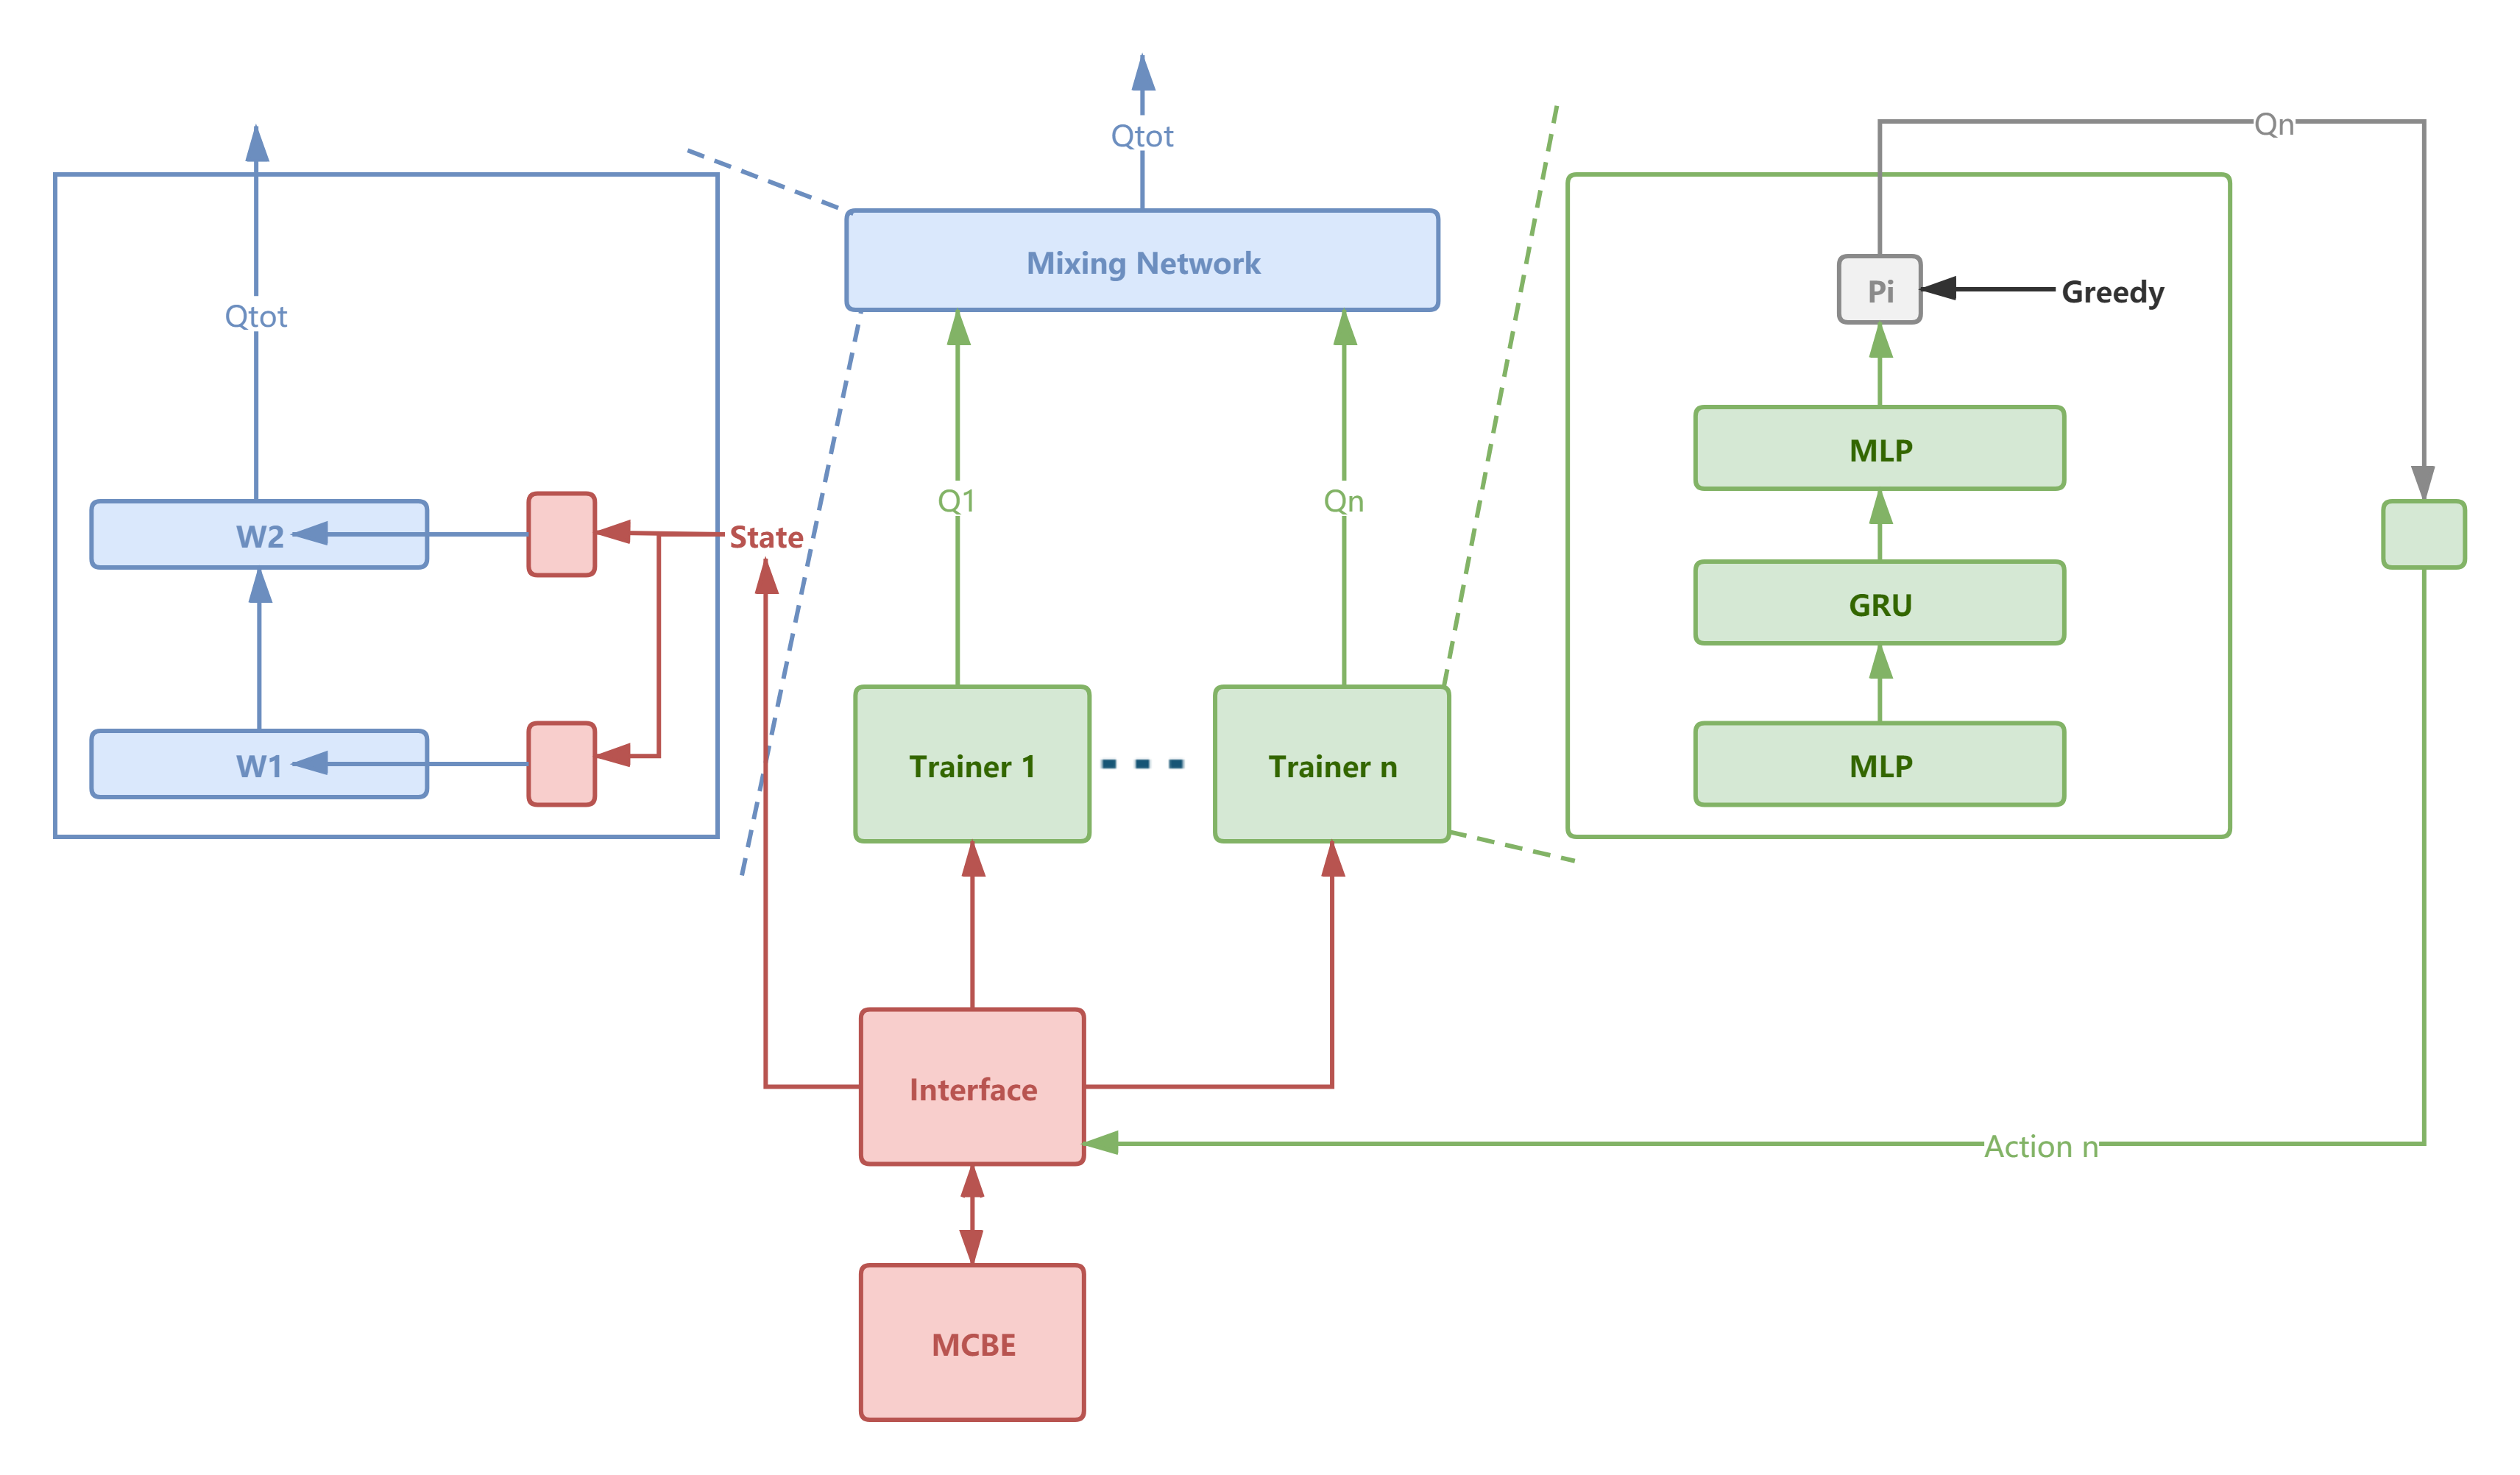
\includegraphics[width=0.80\textwidth]{./images/scml-qmix.png}
\caption{\gls{qmix} used in \gls{mcbe}}
\label{fig:method-qmix-scml}
\end{figure}

\subsection{Experiment}
\subsubsection{Concurrent Neogtiations in standard \gls{scml}}
Standard \gls{scml} is a complex simulation world, which contains various parts with specific functions. The breif description of this simulation is introduced in chapter Background \ref{background-scml}. The experiment of this thesis focus on only the Negotiation Manager of Decision-Maker Agent. The above mentioned method maddpg \ref{methods:maddpg} is used in this experiment. 
Scenario is diagramed in Figure \ref{fig:scenario-standar-scml}

\begin{figure}[htbp]
\centering
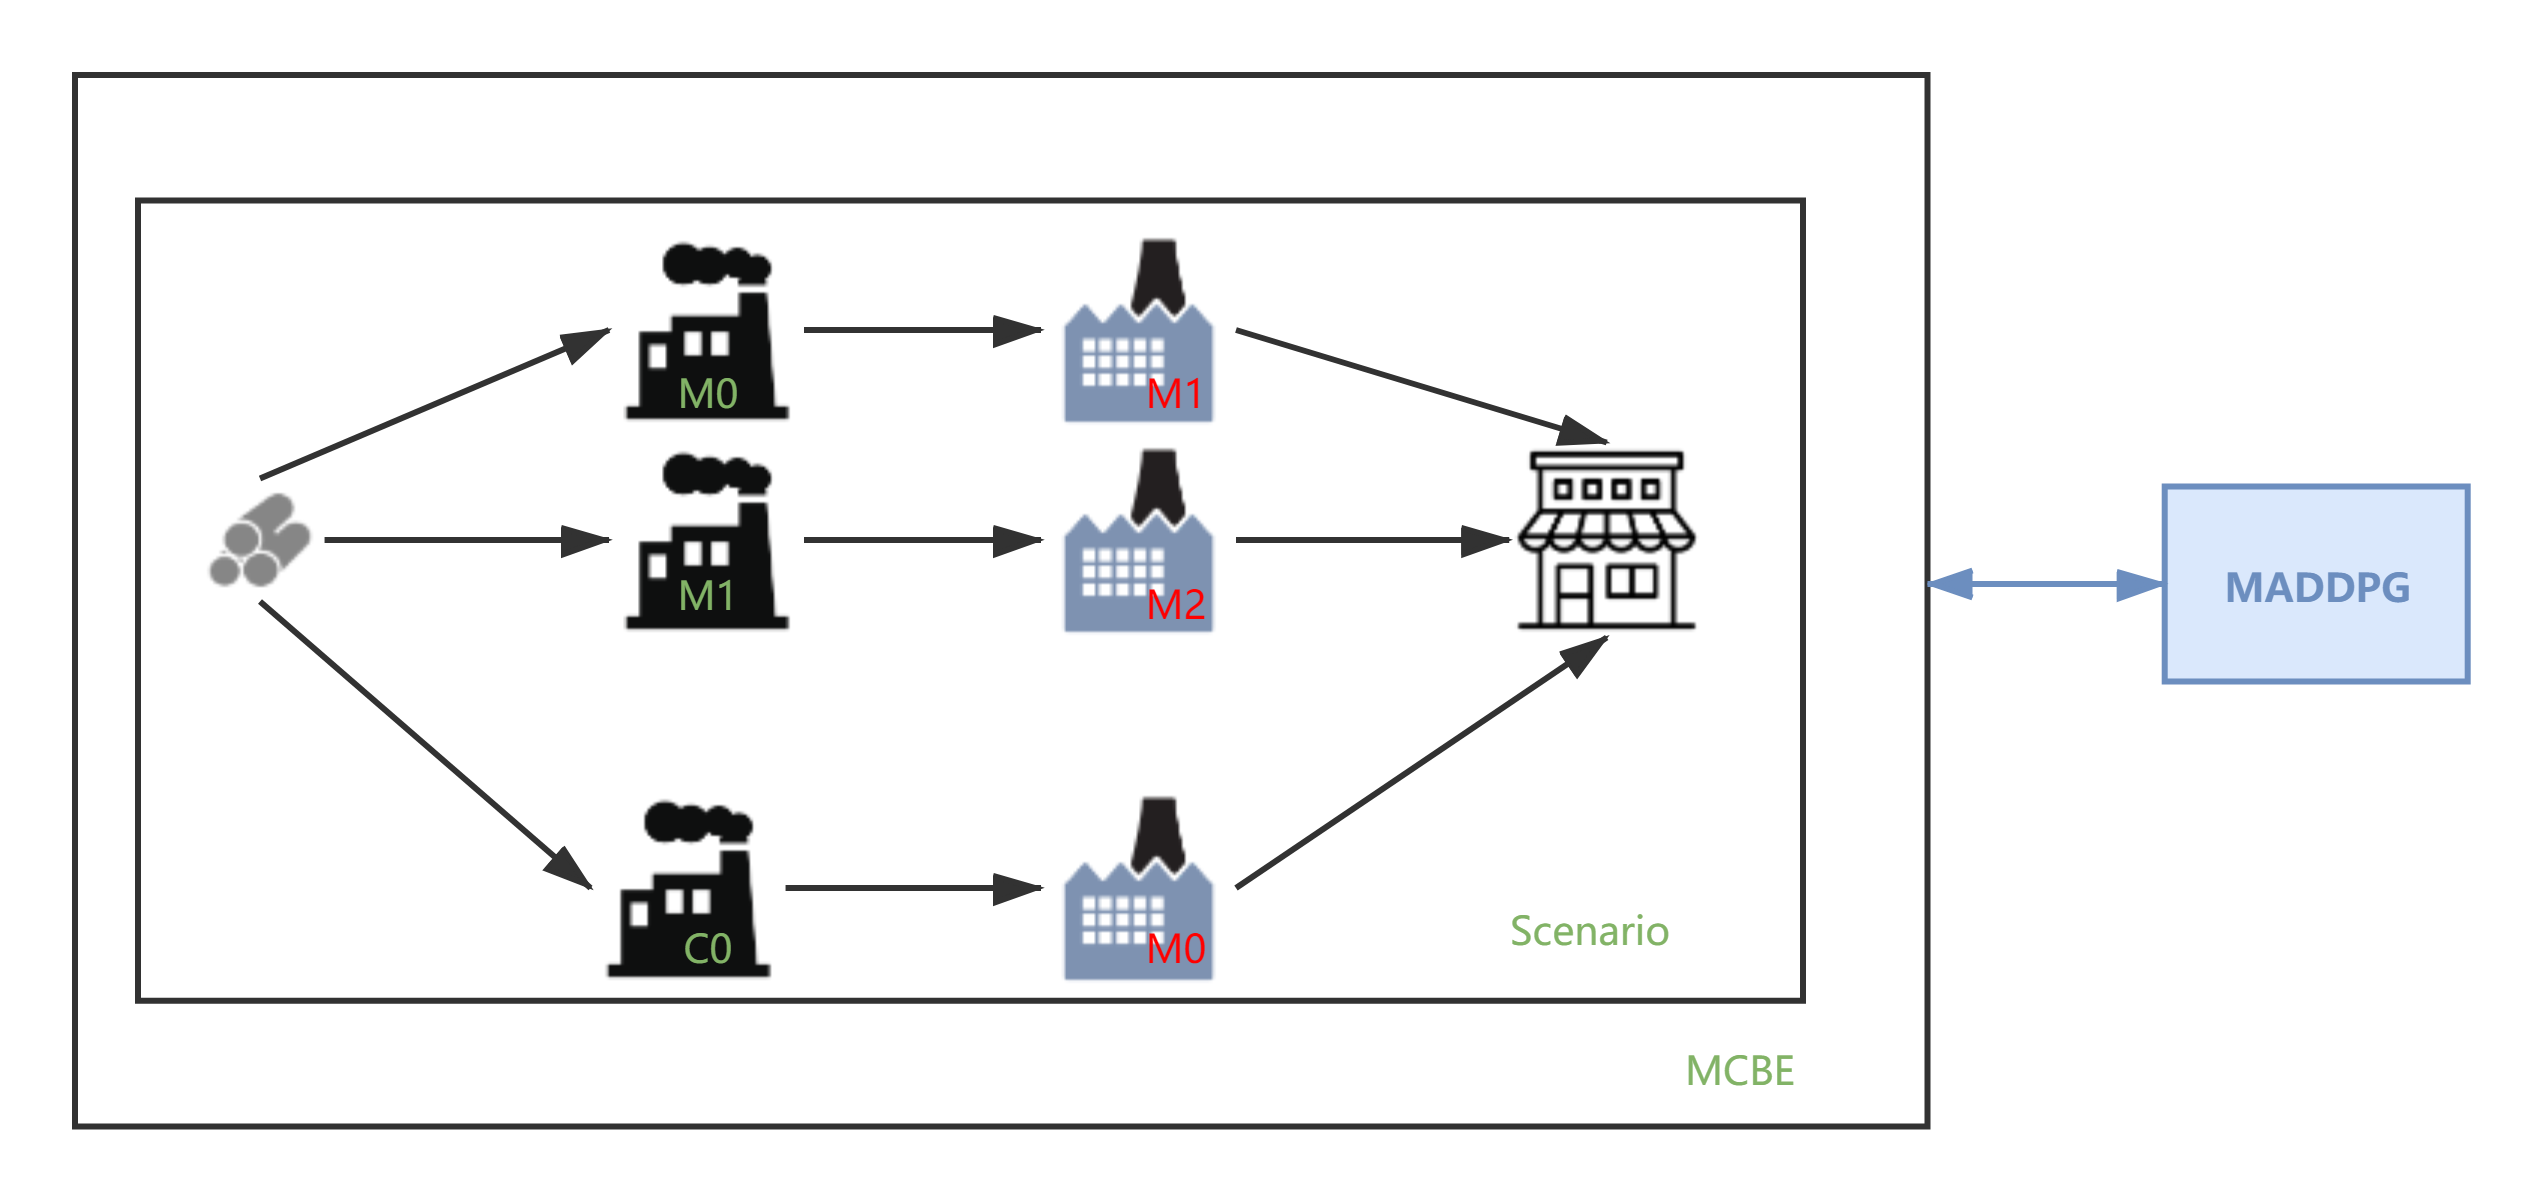
\includegraphics[width=0.80\textwidth]{./images/scenario-standar-scml.png}
\caption{M* represent My Component Based Agent with learner \gls{maddpg}, C* represent Opponent Agents, such as \gls{ind-dec-agent}}
\label{fig:scenario-standar-scml}
\end{figure}

\paragraph{Evaluation} Before evaluating the result of concurrent bilateral negotiation with \gls{maddpg} in standard \gls{scml}. The result of a simple pre-test version which changes the range of negotiation issues with \gls{maddpg}
is shown in \ref{fig:dynamical-range-issues-maddpg}.

\begin{figure}[htbp]
\centering
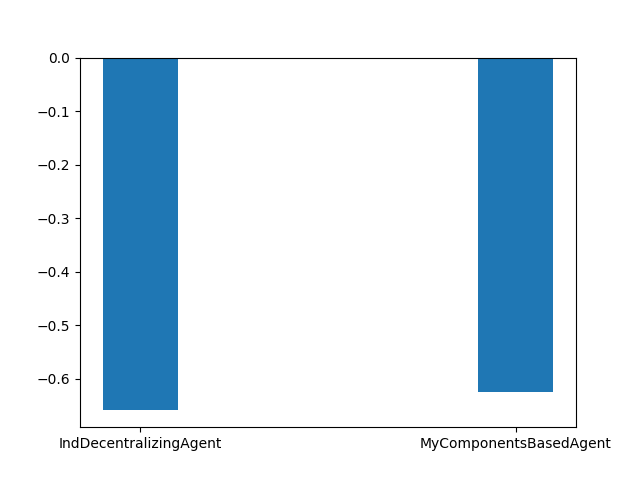
\includegraphics[width=0.80\textwidth]{./images/dynamic_range_issues_maddpg.png}
\caption{}
\label{fig:dynamical-range-issues-maddpg}
\end{figure}


\subsubsection{Concurrent Negotiations in OneShot \gls{scml}}
\textbf{self-play}

Episode mean reward curve is shown in \ref{fig:oneshot-self-play}

\begin{figure}[htbp]
\centering
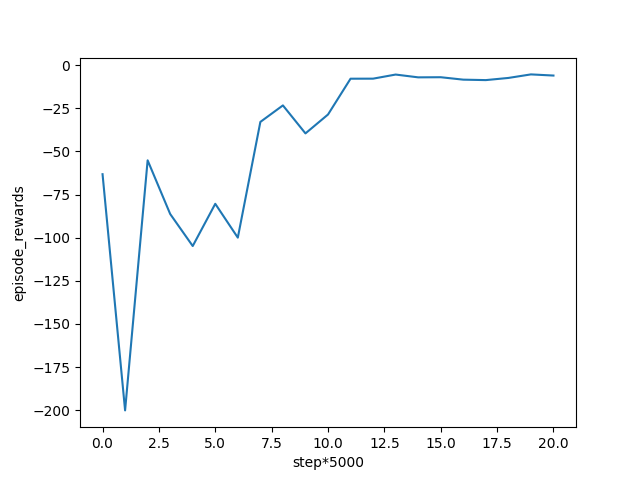
\includegraphics[width=0.80\textwidth]{./images/oneshot_self_play.png}
\caption{Episode mean reward of self paly under SCML OneShot}
\label{fig:oneshot-self-play}
\end{figure}

\textbf{play with other agent}

My agent vs GreedyOneShotAgent

Episode mean reward curve is shown in \ref{fig:oneshot-my-vs-greedy}

\begin{figure}[htbp]
\centering
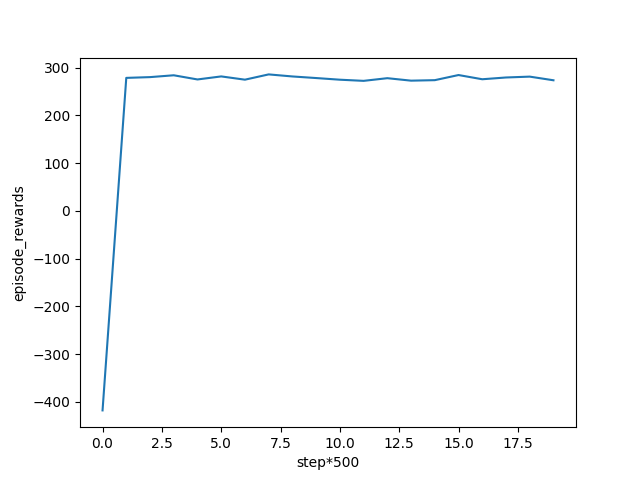
\includegraphics[width=0.80\textwidth]{./images/oneshot_my_vs_greedy.png}
\caption{Episode mean reward of my agent vs GreedyOneShotAgent under SCML OneShot}
\label{fig:oneshot-my-vs-greedy}
\end{figure}

\paragraph{Evaluation}


\section{Conclusion}